
\chapter{Implementation}
\label{sec:implementation}
\noindent

In this chapter, we provide a detailed implementation of our proposed methodology. We start with presenting the platform we incorporated to shape and design our model. Then we demonstrate our network's architecture in detail. Finally, we attempt to give insight into the datasets we used to train and test our model. 

\section{Caffe deep learning platform}

Caffe is a clean and modifiable framework for state-of-the-art deep learning algorithms and a collection of reference models. The framework is a BSD-licensed C++ library with Python and MATLAB bindings for training and deploying general-purpose convolutional neural networks and other deep models efficiently on commodity architectures. It powers on-going research projects and large-scale industrial applications in vision, speech and multimedia by CUDA GPU computation (CUDA is a parallel computing platform and application programming interface (API) model created by NVIDIA\cite{cuda}), processing over 40 million images a day on a single K40 or Titan GPU\cite{jia2014caffe}. 
The main components of Caffe architecture are listed and succinctly explained in below:
\begin{enumerate}
\item \textbf{Data storage:} Caffe stores and communicates data in 4-dimensional arrays called \textit{blobs}. Blobs provide a unified memory interface, holding batches of data, parameters, or parameter updates. Blobs conceal the computational overhead by synchronizing from the CPU host to the GPU device as needed. Caffe supports some data sources such as LevelDB or LMDB, HDF5, MemoryData, ImageData, etc. However, large-scale data is stored in LevelDB data bases since it reads the data directly from memory\cite{caffe}. 
\item \textbf{Layers:} A caffe layer takes blobs as input and yields one or more as output. In a network, each layer plays two important roles: a forward pass that takes the inputs and produces the outputs, and a backward pass that takes the gradient with respect to the output, and computes the gradients with respect to the parameters and to the inputs, which are in turn back-propagated to earlier layers \cite{jia2014caffe}.

\indent Caffe affords a exhaustive set of layers including: convolution, pooling, fully connected, nonlinearities like rectified
linear and logistic, local response normalization, element-wise operations, and losses like softmax and hinge \cite{jia2014caffe}.  
\item \textbf{Networks and run mode:} Caffe ensures the correctness of the forward and backward passes for any directed acyclic graph of layers. A typical network begins with a data layer laying at the bottom going up to the loss layer that computes tasks' objectives. The network is run on CPU or GPU independent of the model definition. 
\item \textbf{Training a network:} Training phase in Caffe is done by classical stochastic gradient descent algorithm. When training, images and labels pass through different layers to be fed to the final prediction into a classification layer that produces the loss and gradients which train the whole network. Figure~\ref{fig:caffe} illustrates a typical example of a Caffe network. 

\indent Finetuning, the adaptation of an existing model to new architectures or data, is a standard method in Caffe. Caffe  finetunes the old model weights for the new task and initializes new weights as needed. This capability is essential for tasks such as knowledge transfer \cite{donahue2013decaf}, object detection \cite{girshick2014rich}, and object retrieval \cite{guadarrama2014open} \cite{jia2014caffe}.  
\end{enumerate}

\begin{figure}[H]
	\centering
	{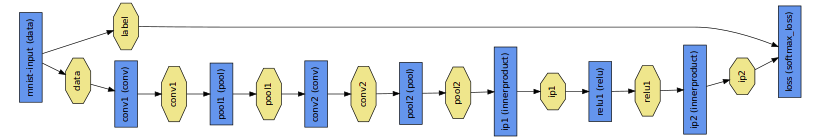
\includegraphics[width=1\textwidth]{images/caffe}}
	\caption{An MNIST digit classification example of a Caffe network, where blue boxes represent layers and yellow octagons represent data blobs produced by or fed into the layers\cite{jia2014caffe}.}
	\label{fig:caffe}
\end{figure}

We decided to use Caffe because, it addresses computation efficiency problems (as likely the fastest available implementation of deep learning frameworks), adheres to software engineering best practices, providing unit tests for correctness and experimental rigor and speed for deployment. It is also well-suited for research use,due to the careful modularity of the code, and the clean separation of network definition (usually the novel part of deep learning research) from actual implementation\cite{jia2014caffe}. Moreover, providing Python wrapper which exposes the solver module for easy prototyping of new training procedures. 

\section{The architecture}

In learning features or object representations for vision tasks and by the use of neural networks, the depth of network plays an important role. The deeper the model, the better it learns. However, issues like overfitting and underfitting should not be left neglected.   
Having Caffe platform introduced, we propose the designed network for two experiments we did regarding learning to count problems. Therefore, in this section, networks' settings and architectures for even digit recognition and crowd counting problems will be described separately. 

\subsection{Even digit recognition}

For learning to count even digits problem, since we used MNIST dataset to generate our dataset, we decided to start with an architecture similar to the classic MNIST hand-written digit recognition problem\cite{lecun1995comparison}. From there, we modified the architecture so that we can optimize the performance. The selected model obtaining the best results, has the following settings and design. 
 
\begin{figure}[]
	\centering
	{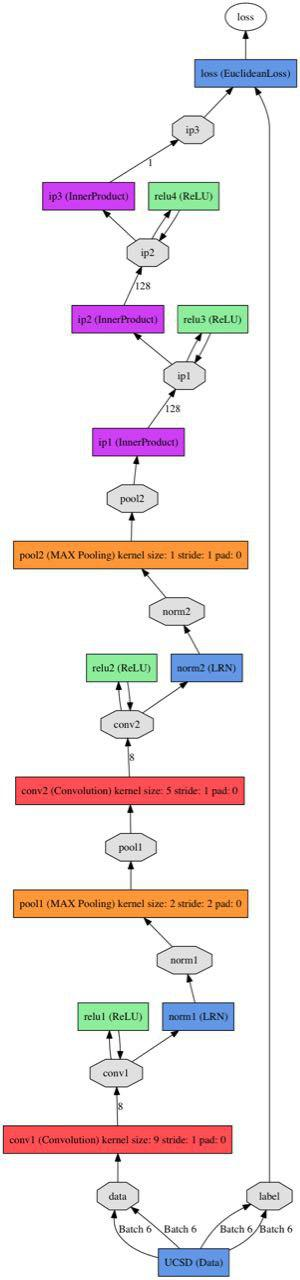
\includegraphics[width=0.3\textwidth]{images/model}}
	\caption{An MNIST digit classification example of a Caffe network, where blue boxes represent layers and yellow octagons represent data blobs produced by or fed into the layers\cite{jia2014caffe}.}
	\label{fig:caffe}
\end{figure}

\begin{figure}[H]
 \begin{flushright}% or better \raggedleft see comments below
  {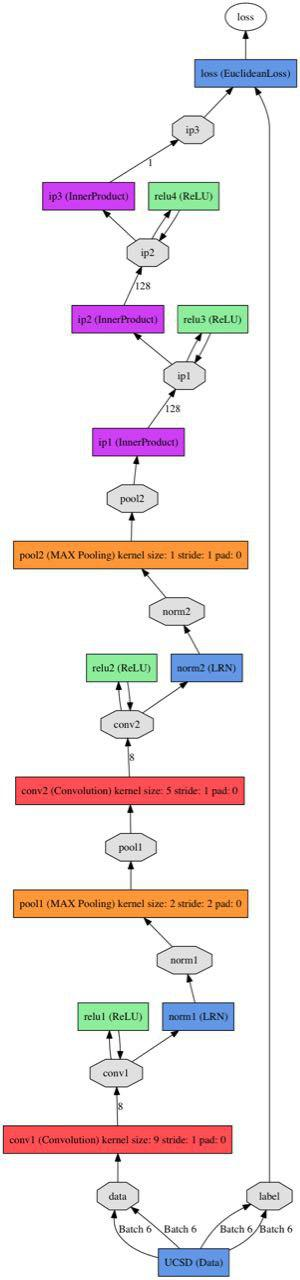
\includegraphics[width=0.2\textwidth]{images/model}}
	\caption{An MNIST digit classification example of a Caffe network, where blue boxes represent layers and yellow octagons represent data blobs produced by or fed into the layers\cite{jia2014caffe}.}
 \end{flushright}
\end{figure}



\subsection{Crowd counting}

